\chapter{ELEMENTARY TRANSPOSITION SYSTEMS}

 

\section{SIMPLE MONOLITERAL TRANSPOSITION METHODS}

\subsection{Transposition Ciphers in General}

Transposition ciphers are like “jig-saw puzzles” in that all the pieces
of which the whole original is composed are present but are merely disarranged. The pieces into which the picture forming the basis of' a jig-saw puzzle may be divided are irregular in size and shape, but the pieces
into which the plain text forming the basis of a transposition cipher may
be divided must be much more regular, for the sake of practicability.
They must be either single letters or pairs of letters, or sets of letters in
regular groupings, or, in an exceptional case, whole words. Most transposition methods however, deal with individual letters and are therefore
termed “monoliteral methods.” The other methods are termed ”polyliteral
methods.”

\subsection{Geometric Designs}

\mypara Practically all monoliteral or polyliteral transposition ciphers involve
the use of a design or geometric figure, such as a square, rectangle, tri—
angle, trapezoid, etc., in which the letters of the plain text are first
inscribed or written according to a previously agreed upon direction of
writing and then transcribed or rewritten according to another and different, previously agreed-upon direction to form the text of the cryptogram.
In nearly all cases the specific key consists in (1) using designs of a specific nature and dimensions, and (2) varying the direction or manner of
inscription or transcription, or both.

\mypara In working with transposition ciphers or, for that matter, most
types of ciphers, cross—section paper will be found very convenient.
Cross-section paper with M-inch squares is most suitable. For brevity in
reference, the individual small squares of such cross-section paper will
hereafter be called cells.

\subsection{Route Transpositions}

\mypara. Suppose the correspondents agree to use the method of monoliteral
transposition known as route transpgsition, The message is inscribed 
within a rectangle in the usu-al manner of writing, that is, from left to
right and in consecutive lines from top to bottom. If one or more cells
are vacant at the end, nulls or dummy letters—letters having no significance—are inserted as “fillers” to complete the rectangle. Then, to form
the cipher text, the letters in the design are taken out of the design and
rewritten or transcribed by following or tracing one of many different
routes. It is possible for each route to have a difl’erent starting point, and
normally it is one of the four corners of the rectangle. A few typical
routes are illustrated in \ref{fig:Figure 1} where, for the sake of ease in following
the route, the plain—text message is assumed to be merely the sequence
of letters A B C X.

\begin{figure}[h]
  \centering
    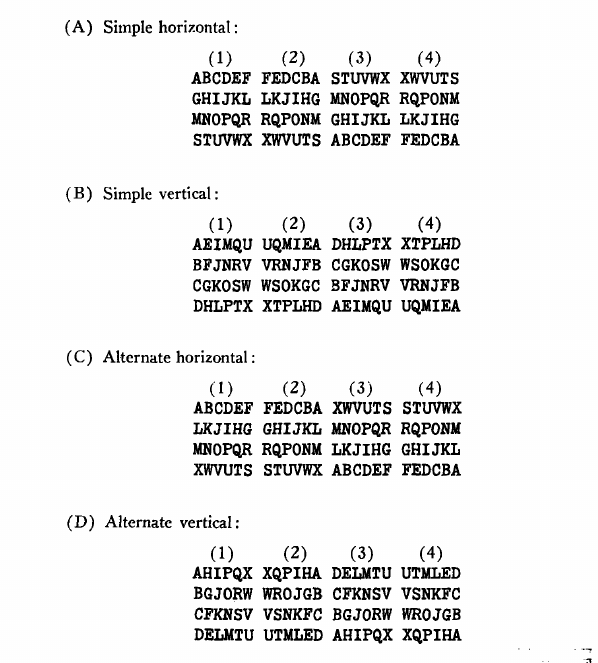
\includegraphics[width=0.7\textwidth,natwidth=598,natheight=663]{Chapter2_fig1.png}
    \caption{Figure 1}
    \label{fig:Figure 1}
\end{figure}

\begin{figure}[h]
  \centering
    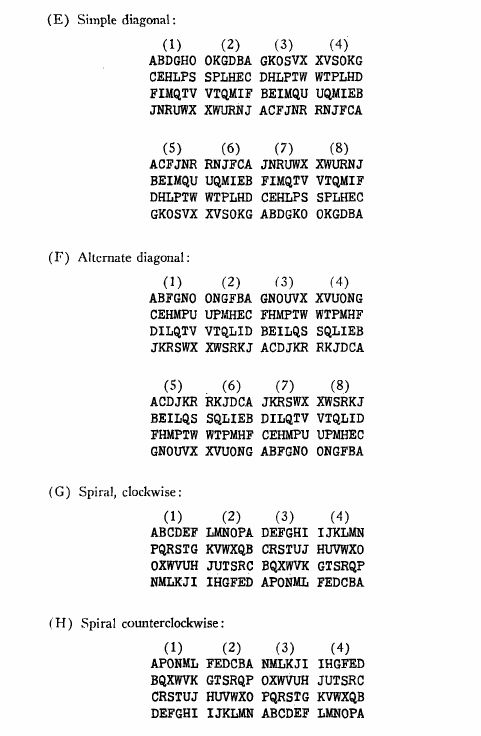
\includegraphics[width=0.6\textwidth,natwidth=481,natheight=736]{Chapter2_fig1Continued.png}
    \caption{Figure 1 continued}
\end{figure}


\mypara It is apparent that instead of following the normal direction of
writing, that is, from left to right and from the top downwards, the
letters of the plain text may be inscribed according to any one of the
routes agreed upon, and then transcribed to form the cipher text by
taking the letters from the rectangle in the normal manner, that is,. in
this case from left to right, and from the top downwards, or by following any other route of transposition.

\subsection{Example of Encipherment and Decipherment by Monolilteral Route Transposition}

\mypara Now take a special example of encipherment by monoliteral route
transposition. Use the message ATTACK HAS BEEN POSTPONED
UNTIL TOMORROW TWO AM, and employ a relatively cemplicated
method. Suppose that the general system agreed upon is the one being
described, and that the specific key consists of the following elements:

\begin{enumerate}
\item Using a completely filled rectangle of seven columns;

\item Inscribing the letters of the plain text within the rectangle by
following route (F) (3) of \ref{fig:Figure 1}.

\item Transcribing the thus inscribed letters (to form the cipher text)
by following route (E) (6) of \ref{fig:Figure 1}.
\end{enumerate}

Since the message contains a total of 40 letters, and it has been
agreed to use a completely filled rectangle of seven columns, it is
necessary to add two nulls to make the total numberof letters a
multiple of seven. A rectangle of seven columns of cells and six
lines of cells is therefore prepared. The design is then filled in as
shown in \ref{fig:Figure 2}.

\mypara To decryptograph such a cryptogram the process is merely reversed.
First, the total number of letters in the cipher text must be found. Since

\begin{figure}[h]
  \centering
    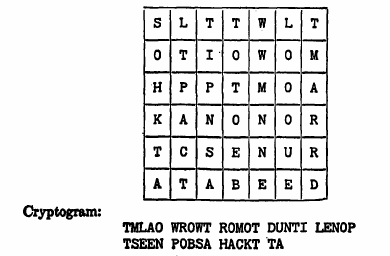
\includegraphics[width=0.6\textwidth,natwidth=390,natheight=256]{Chapter2_Figure2.png}
    \label{fig:Figure 2}
    \caption{Figure 2}
\end{figure}

it is 42, and since a completely filled rectangle of seven columns has been
agreed upon, a design consisting of seven columns and six rows is outlined on cross-section paper. The cipher text is then inscribed according
to route (E) (6) of \ref{fig:Figure 1}, and after this has been completed the plaintext letters are read according to route (F) (3), \ref{fig:Figure 1}. It is apparent
that it is necessary to remember a relatively long series of rules, and even
when the cryptographing has been accomplished correctly the degree of
security is very low. Note how obviously the whole word UNTIL mani—
fests itself in the cipher text. Parts of other words can also be seen.
The degree of security remains very low despite the variability afforded
by the dimensions of the rectangle, the method of inscription and transcription and their starting points.

\subsection{Use of Nulls in Transposition}

\mypara It will be noted that the two nulls selected as fillers to complete the
rectangle in the preceding example were the letters L and T. These were
chosen rather than such letters as J, K, Q, X, or Z, for a reason which
is important to note. Since transposition ciphers of this type involve
merely a rearrangement of the letters, without any change whatever in
their identities, it follows that the natural or normal frequencies of letters
of plain text remain unchanged. Now, the letters of every alphabetic
language have characteristic frequencies, as a result of which certain clues
are afforded in cryptanalysis. The presence, in transposition ciphers, of
letters of very low frequency (in English), such as J, K, Q, X, or Z, is
very unusual and therefore if these are employed merely as fillers they
may afi'ord clues as to the real number of letters in the plain text, the
starting or finishing points of the real text, etc. For this reason it is best
to insert as fillers in transposition ciphers letters of medium or high fre—
quency, such as E, T, R, I, N, O, A, S, D, L, or C, for thesct' will not
afford any clues to solution. Nulls, when employed for the purpose of
making cryptanalysis more difficult, may also be inserted in specific positions as prearranged, or they may be inserted at random if the system
permits. This is true of other cryptographic systems, but as a general
rule the use of nulls, especially in cipher systems, is to be discouraged.
Very often they add little if any security, and thus merely increase the
length of the cryptographic text without any compensating advantages.

\mypara Whenever it is necessary to add nulls in order to complete a transposition message in any respect, or for any reason whatsoever, they must
be added before the transposition process is applied and not afterward;
otherwise it will be difficult or even impossible for the decryptographing
clerk to read the message. This is especially true when the service regulations require that the final group in a cryptogram be a complete group,
containing exactly as many letters as all other groups in the message.


\subsection{Special Cases of Route Transposition}

\mypara The oldest and simplest transposition method known, that called reversed writing, is a special case of one of the routes shown in \ref{fig:Figure 1}.
Here the text is written in the opposite direction from the normal; for
example, BRIDGE DESTROYED is written EGDIRB DEYORTSED.
The variability of the scheme, that is, the specific key, consists of the fact
that the reversal may be applied to groups of fixed length, to whole
words, to sentences, or to the whole text. The security of simple reversed
writing may be somewhat increased by disguising the original word
lengths, by which is meant a destruction of the normal, or natural word
limits by combining a part of one word with a part of the next to form
either false words or groups of regular length.

\mypara Some examples of reversed writing follow. Let the message be:
BRIDGE DESTROYED AT ELEVEN PM.

\begin{enumerate}
\item Reversing only the words and retaining original word lengths:
Cipher: EGDIRB DEYORTSED TA NEVELE MP
\item Reversing only the words and regrouping into false word
lengths:
Cipher: EG DIRB DEYOR'I‘ SEDTA NEVE LEMI>
\item Reversing the whole text and regrouping into fives:
Cipher: MPNEV ELETA DEYOR TSEDE GDIRB
\item Reversing the whole text, regrouping into fives, and inserting
a null in every fifth position:
Cipher: MPNER VELEO TADEB YORTH SEDEA GDIRB
\end{enumerate}

\mypara A second very simple type of transposition, that known as vertical
writing, is a special case of another of the routes shown in \ref{fig:Figure 1}.

The message BRIDGE DESTROYED is written in two vertical
columns, and the cipher text is taken from the horizontal pairs
thus formed. The message becomes:

\begin{figure}[h]
  \centering
    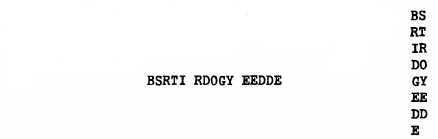
\includegraphics[width=0.8\textwidth,natwidth=438,natheight=139]{Chapter2_Figure3.png}
    \label{fig:Figure 3}
    \caption{Figure 3}
\end{figure}

When the plain text is inscribed in pairs of letters in vertical
writing and then the cipher text is taken by transcribing the
columns, a slightly different result is obtained. Using the plain
text message BRIDGE DESTROYED, the cipher becomes:

BIGDS RYDRD EETOE R0

Figure 4.

This type of transposition is sometimes Called the \textit{rail-fence} cipher
because it can be produced by writing the message in the following form:

BIGDSRYD
RDEETOE

which yields the same cipher result as before.

\subsection{Remarks on Monoliteral Route Transposition}

Reversed writing and vertical writing of the types indicated yield ex-
tremely simple cryptograms. In practice they are sometimes used in con—
nection with other more or less simple cryptographing methods to in-
crease their security. The cryptographic security of the other methods
thus far indicated is also very low, despite the apparently large degree of
variability they afford. The reason is that the route to be followed in the
inscription or transcription process is definitely fixed under each type of
route. In other types Of transposition soon to be discussed, a much
wider latitude for variation in the route is afforded by the use of- kley
words to control or to guide these processes. Geometric designs are also
used in these types of transposition, and key words determine the dimen-
sions of the design, or else, if only one key word is used, it determines
one dimension, the other being determined by the length of the text.
Examples given in their proper place will serve to illustrate the processes.

\subsection{Key Words and Numerical Keys}

\mypara It is often necessary, in performing certain cryptographic operations, to employ a numerical key, which may consist of a relatively long
sequence of numbers difficult or impossible for the average cipher clerk
to'memorize. To avoid making it necessary that such sequences of numbers be carried on the person in written form, a dangerous procedure,
cryptographers have devised very simple methods of deriving such
sequences from words, phrases, or sentences, which can usually be remembered much more easily than can unintelligible, relatively long sequences of numbers. One of the simplest methods is to assign numerical
values to the letters of the key in accordance with their relative positions
in the ordinary alphabet. Such a key is called a derived numerical key.
This method of assigning the numbers is very flexible and varies with
different uses to which numerical keys are put. For purposes of transposition, the method shown below is very satisfactory. .

\mypara Let the prearranged key word be the word CARBUNCLE. Since
the word contains the letter A, which comes first in the alphabet, the
number 1 is written under this letter in the key word. Thus:

CARBUNCLE
 1


The next letter of the normal alphabet that occurs in the key word is B,
which is assigned the number 2. The letter C, which occurs twice in the
key word, is assigned the number 3 for its first occurrence, the number 4
for its second occurrence, and so on. The final result is:

Basic key word: C-A-R-B-U—N-C-L-E
Derived numerical key: 3-1-8-2-9-7-4-6-5

\mypara The method may, of course, be applied tophrases or. to- sentences,
so that a. very long numerical key, impossible ordinarily to remember,
may be so derived at will from an easily remembered key text.

\mypara It is advisable to make note of a few points valuable 1n connection
with the choice of key text:

\begin{enumerate}
\item It should be such as can be easily remembered. Often a key
composed of two or more short words is better than one con-
sisting of a single long word. Thus, the whole sentence WHEN
DO WE EAT would be better than the single word
EXTRAORDINARY.

\item It should consist of one or more simple, familiar words admitting of but one spelling. A word such as REINFORCEMENT
is inadvisable because the spelling REENFORCEMENT is
also admissible. It goes almost without saying the use of words
suitable for “spelling bees,” even though they may be familiar,
everyday words as DEFINITELY, SEPARATELY, REPETITION, etc. is likewise inadvisable.

\item It should contain as many different letters as possible, in no
systematic sequence. Words with several repeated letters, such
as ELEMENT, BANANA, MISSISSIPPI, etc., form poor
key words.

\item It should present no associations with the special situation in
which it is used, so as not to be easily guessed by the enemy.
For example, to use personal or geographic names associated
with a region in the theater of operations is bad practice. The
key word GETTYSBURG employed in a cryptogram originat-
ing in the vicinity of Gettysburg would be bad practice. Or to
use for this purpose words of common military usage, such as
BATTALION, REGIMENT, ARTILLERY, SIGNAL
CORPS, MACHINE GUN, etc., is likewise bad practice.
\end{enumerate}

\mypara It is convenient to designate key text in letters as a literal key. As
noted, a literal key may consist of a single letter, a single word, a phrase,
a sentence, whole paragraph, or even a book. The method of deriving
a numerical key from a literal key given in b above is only one of a number of methods, but it IS the most commonly employed. It is also subject to
variation in detail. But, so far as the cryptanalyst is concerned, just how
the numerical key is derived from a specific literal key is usually of
interest to him only if this knowledge will assist in subsequent solutions
of cryptograms prepared according to the same basic system. Often the
cryptanalyst is wholly unconcerned as to whether a literal or a numerical
key has been used in connection with cryptographing of the messages,
and he may frequently be unaware of the fact that a literal key has been
used as the basis for deriving a numerical key.

\section{COLUMNAR TRANSPOSITION METHODS}

\subsection{Columnar Transposition with Completely Filled Rectangles}

\mypara One of the most common types of transposition involving the use
of a key word or a derived numerical key is that known as keyed or
variable-key columnar transposition. In this type the letters are usually
written in a geometric design, most often a rectangle, by inscribing them
in the ordinary manner, that is, in horizontal lines from left to right and
from the top downwards, and then the letters are transcribed by
“reading” the columns in the sequence determined by the numerical key.
If the text does not contain a sufficient number of letters to fill the last
line completely, as many nulls as are necessary to do so are added at the
end. Figure 5 is an example of cryptographing by this method.

 

 

 

 

 

 

 

Keyword: L-I-B-E-R-T-Y
Numericalkey: 4-5-1-2-5-6-7
R E P 0 R T L
o c A'T I o N
0 F S E C 0 N
D B A T '1' A L
I 0 N C 0 M M
A N D P 0 S T
T 0 D A Y D N

 

 

 

 

 

 

 

 

 

Note. The letters D and N in the final two cells are nulls, inserted to complete
the rectangle.

Cryptogram :

PASAN DDOTE TCPAE CFBON OROOD IATRI CTOOY
TOOAM SDLNN LMTN

Figure 5.

\mypara To decryptograph such a cryptogram, a rectangle with the proper
number of cells, determined by the length of the message and the length
of the key, must first be prepared. In the foregoing example, since the
cipher text consists of 49 letters and the key consists of 7 letters or numbers, the rectangle shown in (a) of figure 6 is prepared and then the
columns (of cells) are filled in numerical order. An early stage in the
decryptographing is represented in (b) of figure 6. It is only after the
process has been finished that the complete message reappears, as shown
in (c) of figure 6.

Cryptogram :

PASAN DDOTE TCPAE CFBON OROOD IATRI OTOOY T00“
SDLNN LMTN

4-3-1-2—5-6-7 4—3-1-2-5-6-7

(a)
(b)

- (c)

The letters D and N are recognized as nulls.
 

Figure 6



\mypara The method indicated above may vary considerably by changing
(1) the key word, (2) the route followed in inscribing the letters of the
plain text, and (3) the route followed in transcribing them to form the
cipher text. A change in key daily, or oftener, is possible; or, by drawing
up a whole list of daily keys for a given period, automatic change in key
can be provided for without indicating in the cryptograms the applicable
key. It is also possible to prepare a long list of suitable keys and to
designate each key by an indicator inserted in the cryptogram in a prearranged position. Indicators may be words, numbers, groups of letters,
or single letters. For example, each key in a list of 500 may be indicated
by a single pair of letters inserted at the beginning, at the end, or at any
prearranged position of the cryptogram. This procedure has a disadvantage, however: if an error occurs at the particular position of the cryptogram containing the indicator, the decryptographing is made difficult if
not impossible. For this reason indicators, if used, are often inserted
in at least two positions in the cryptogram, usually at or near the
beginning and end.

\mypara The letters of the plain text may be inscribed in the rectangle
according to any one of the routes indicated in \ref{fig:Figure 1}. If the transcribing process is accomplished by reading whole columns or whole
rows, according to a prearranged plan which follows a route perpendicular to the inscribing route (except in the case of spiral inscription), the
decryptographing process is simple. Only certain of the simpler combinations of inscription and transcription are 'suitable for military use, the
most practicable being those illustrated in figures 5 and 6.

\subsection{Columnar Transposition with lncompletely Filled Rectangles}

\mypara The degree of cryptographic security of columnar transposition is
much increased if the rectangle is not completely filled. It is impossible
to go into the reasons for this increased security without demonstrating
solutions; suffice it to say that the solution will be more difficult than
would be suspected if one or more cells are vacant in the last row of the
rectangle. An example of cryptographing and decryptographing is shown
in figure 7.

\mypara To decryptograph such a cryptogram one must first count the
number of letters in the text and then outline on cross-section paper a
rectangle which will exactly contain the message, crossing off the cells
which must remain vacant. In the foregoing example, the text contains
30 letters and, since the key contains 7 letters, the outlined rectangle is as
shown in figure 8 of (a). From the complete rectangle 7 X S = 35 cells,
5 cells must remain vacant at the end.

\mypara The cipher text is then inserted in key—number order, the result of
inserting the first two groups of the text being shown in (b), figure 8.
It is only after the process has been finished that the complete message
becomes apparent.

Message:
REQUEST IMMEDIATE REENFORCEMENTS
Keyword: P-R—O—D—U-C-T
Numericalkey: 4-5-5-2—7-1—6
R E Q U E S T
I M M E D I A '
T E R E E N F
0 R C E M E N
T S
Cryptogram:
SINEU EEEQM RCRIT OTEME RSTAF' NEDEM
Figure 7.

Cryptogram:

SINEU EEEQM RCRIT OTEME RSTAF NEDEM
4-5-3-2-7—1—6 '4—5-5—2—7—1—6

Figure 8.

\subsection{Modification of Columnar Method}

A variation of the columnar procedure, but one that produces exactly
the same results, may be found useful. First, write the message in groups
corresponding to the length of the key. Thus, using the same key and
message as in paragraph 28, the following is obtained:

4-5-3-2-7-1-6 4-5-5-2-7-1-6 4-5-3—2-7-1-6 4-5-

REQUEST IMMEDIA TEREENF 0R

4-5

T S

The letters are then taken from the groups and are transcribed in groups
of five, all letters marked 1 being taken first, then all those marked 2, and
so on. Thus, the first two cipher text groups are SINEU EEEQM,
and the complete text is identical with that produced in figure 7.

\subsection{Addition of Nulls to Complete a Final Group}

The example given in the preceding case happened to contain 30 letters,
a number that is an exact multiple of five. Thus, the final group in the
cryptogram automatically became a complete group. For accuracy, the
final group of every message should be complete; therefore, if the number of letters in the text of a message is not a multiple of five, it should
be made so by the addition of nulls, before the transposition process
is applied (see par. 23b).

\section{MISCELLANEOUS TRANSPOSITIOlN METHODS}
\subsection{Transposition Systems Employing Special Designs}

\mypara Triangles, trapezoids, and other polygons are among the many
designs used to produce transposition ciphers. Most of them, however,
are impractical for wide military use but are used occasionally by secret
agents.

\mypara A grille is a common transposition device of some practical importance. There are several types and one of the most common is that known
as the rotating grille. It is usually made of a square sheet of cross-section paper from which cells have been cut in definite but apparently
irregular positions. The grille is superimposed on another sheet of crosssection paper of the same dimensions and the letters of the message are
written in the cells exposed by the perforations. Usually the grille is
then given a 90° turn clockwise or counterclockwise, as agreed, and the
fresh cells exposed by the perforations are filled with the next few letters
of the text. If the grille has been prepared properly it is possible to give it
four turns of 90° each, at the end of which all the cells on the under
sheet of cross-section paper are occupied by letters. The grille is then
removed and the letters of the sheet underneath it are transcribed in
accordance with some prearranged route to form the cipher text. Naturally, the correspondents must have identical grilles and every. step must
be definitely prearranged. Although it is possible to construct grilles with
many different arrangements of perforations, the necessity for carrying
the device on the person, and the many agreements and understandings
necessary for its successful operation make the method hardly suitable
for field military use. Furthermore, practical difficulties connected with
the preparation and distribution of many grilles would make it almost
inevitable that several messages would be enciphered by the same grille.
The degree of cryptographic security aflorded by them is not so great as
may be suspected; sometimes single messages of fair length may
be solved.

\subsection{Polyliteral and Word Transposition}

\mypara Thus far only individual letters, as units for the transposition
process have been discussed. It is possible to use pairs of letters, sets of
three or more letters, or entire words as units; procedures are the same
in monoliteral and polyliteral transpositions. Sometimes more complicated
routes may be followed in transposition; for example, a route may be a
prearranged succession of moves made by a knight in chess. It is usually
necessary to have at hand a printed form showing the complete route,
and this makes these methods impractical for field use. They may, however, be used in special cases.

\mypara The cipher system used by the Federal Army in the Civil War
represents a good example of word transposition. In the earliest form
in which this cipher was used by the Federals only one route was used,
which consisted in writing the text in six columns, going up the sixth,
down the first, up the fifth, down the second, up the fourth, and down
the third. Arbitrary words were substituted for proper names, nulls were
introduced at regular positions, and words even often misspelled for
further obscurity. For example, the word “operation” was often spelled
as two words: “opera,” and “shun.” Later, many additional routes were
provided, relatively long lists of arbitrary equivalents for names, numbers, dates, common military terms, etc., were added, and the whole
system was made considerably more complicated. While the security
afforded by this system was probably ample for those days, it would
hardly be sufficient today to permit its use even in cases where a delay
of only a few hours is required. Furthermore, if long lists of arbitrary
equivalents must be handled, the system presents all the disadvantages of
a poor cipher system with but few of the advantages offered by a good
code system.

\subsection{Single and Double Transposition Methods}

In single transposition methods the letters go through only one transposition from plain text to cipher text. It is possible to take the letters
resulting from a first transposition and apply a second transposition to
them; cryptograms so prepared often present a very great degree of
security. Triple and quadruple transposition is possible but wholly
impracticable for common use. Only a very limited number of double
transposition methods are practicable for military use, but the degree of
security afforded by certain of them is much greater than that afforded
by certain much more complicated substitution methods.

\subsection{Factors Concerning Use of Transposition Systems}

\mypara The transposition methods described above provide a wide range
of cryptographic security; in some there is very little security, in others
there is a great deal. All transposition systems usually present important
advantages in speed and simplicity. These advantages have led to attempts
to increase security in some manner or other; double transposition
schemes, rotating grilles, and other more complicated methods have consequently been developed. In only certain types are written memoranda
or devices required. Very often the entire cryptographing process in even
very complex methods may be easily memorized by persons of very good
intelligence, such as secret agents. For these reasons transposition systems
are often useful in espionage and counterespionage activities.

\mypara But transposition ciphers for military usage present three very
serious disadvantages. In the first place, the methods are such that they
do not allow any latitude for errors in handling. Often if a single letter
is omitted or added, as not infrequently happens in telegraphic transmission, the whole message becomes difficult if not impossible to decryptograph. In the second place, if two or more messages prepared in the
same key and containing exactly the same number of letters are available
for study, no matter how complicated the method employed, the cryptograms can be solved, and the key recovered, and applied to other
cryptograms in the same key but with different numbers of letters. In
military cryptography it is not unusual, in cases of heavy traflfic, to have
as many as 100 or 200 messages transmitted on the same day, all in the
same key. Control from a central headquarters of the exact message
length would obviously be impossible. The chances, therefore, that the
enemy may actually intercept and find several messages of identical
length are not negligible. Thus, a transposition method presenting an
extremely high degree of cryptographic security when only a few
messages are to be cryptographed fails seriously when employed for
heavy trafiic. Finally, in certain cases, where the double transposition
produces a great degree of security, it is almost inevitable that a poorly
trained or careless cryptographic clerk will fail to perform both steps
correctly. Not only messages prepared by one poor or careless operator,
but all other messages, even though correctly prepared, are thus laid
open to solution.
